\chapter{植物适应与表型可塑性}\label{ch:b2:plant-plasticity}

同一棵橡树上的两片叶子：树冠顶部的那片
小而厚、质地如皮革；树冠内部遮阴处的那片
则是其三倍大，薄如纸。同一棵橡树的幼苗
若生长在郁闭的林冠之下，就长得又高又细；
生长在林间空地上的兄弟幼苗则矮小粗壮。
这些差异都不是遗传造成的。植物不能走到更好的
地方去，因此只能把自身构建成适合所处位置的样子：
它感知光、重力、接触、水分、盐分和低温，并据此
弯曲、增粗、伸长、关闭\omterm{prop:b2:plant-plasticity:stomata}{气孔}或使细胞变硬。
本章讨论的正是这种可塑性——植物如何读取周围环境，
又如何作出反应——以及谱系借以适应沙漠、荫蔽、
盐碱和霜冻的可遗传适应。

\section{可塑性及其限度}

\begin{definition}[表型可塑性与反应规范]\label{def:b2:plant-plasticity:plasticity}
\index{表型可塑性}\index{反应规范}\index{驯化适应}\index{适应}
\emph{\omterm{def:b2:meiosis-heredity:vocabulary}{表型}可塑性}是同一\omterm{def:b2:meiosis-heredity:vocabulary}{基因型}
在不同环境中产生不同\omterm{def:b2:meiosis-heredity:vocabulary}{表型}的能力。\omterm{def:b2:meiosis-heredity:vocabulary}{基因型}的
\emph{反应规范}是其\omterm{def:b2:meiosis-heredity:vocabulary}{表型}随某一环境变量变化的曲线——
例如叶片厚度随光照、茎长随温度的变化。不同\omterm{def:b2:meiosis-heredity:vocabulary}{基因型}
的反应规范各不相同，而即使可塑性本身不可遗传，
这些差异仍是可遗传的。\emph{驯化适应}是可逆的生理形式：
例如一片叶子在干燥的一周里加厚角质层，
一个细胞在秋季合成抗冻物质。\emph{适应}按进化意义理解，
是谱系经世代选择后对其栖息地的可遗传适合性；
仙人掌适应干旱，豆类植物则在短暂干旱中驯化适应。
植物比动物更具可塑性，因为它们
是模块化的、无限生长的（见\cref{ch:b2:plant-meristems}）：
下一片叶子可以与上一片不同地构建，
而固着生活使可塑性成为
植物唯一的“移动”方式。
\end{definition}

\begin{omfigure}
\begin{tikzpicture}
\begin{axis}[
  width=0.72\linewidth, height=5.4cm,
  axis x line=bottom, axis y line=left,
  xmin=0, xmax=100, ymin=0, ymax=1.2,
  xlabel={光照（占全日照的 \%）}, ylabel={叶片厚度（相对值）},
  xlabel style={font=\small, at={(axis description cs:0.5,-0.13)}, anchor=north},
  ylabel style={font=\small},
  tick label style={font=\small}, xtick={0,25,50,75,100}, ytick={0,0.5,1},
  legend style={font=\scriptsize, at={(0.97,0.08)}, anchor=south east, draw=none},
  clip=false,
]
\addplot[very thick, omDef, domain=2:100, samples=60] {0.35 + 0.65*(1-exp(-x/30))};
\addlegendentry{基因型 1：可塑性强的橡树}
\addplot[very thick, omThm, domain=2:100, samples=60] {0.55 + 0.2*(1-exp(-x/30))};
\addlegendentry{基因型 2：可塑性较弱的一种}
\end{axis}
\end{tikzpicture}

{\small 两条\omterm{def:b2:plant-plasticity:plasticity}{反应规范}。每种\omterm{def:b2:meiosis-heredity:vocabulary}{基因型}在光照更强时都会长出更厚的叶片；
曲线的斜率——即可塑性——本身也是一种可遗传性状，
两种\omterm{def:b2:meiosis-heredity:vocabulary}{基因型}在这方面各不相同。}
\end{omfigure}

\begin{proposition}[阳生叶与阴生叶]\label{prop:b2:plant-plasticity:sunshade}
\index{阳生叶}\index{阴生叶}
在全日照下发育的叶片小而厚，具两到三层栅栏细胞、
大量\omterm{prop:b2:plant-plasticity:stomata}{气孔}、厚角质层，
固碳酶浓度高，最大光合速率
也高；同一植株在遮阴处发育的叶片
则大而薄，只有一层栅栏细胞，单位质量的叶绿素更多，
呼吸速率低，光补偿点也低。
\omterm{prop:b2:plant-plasticity:sunshade}{阴生叶}的构造使其能以最低代价捕获每一个光子，
\omterm{prop:b2:plant-plasticity:sunshade}{阳生叶}则能利用大量光子而不致过热或萎蔫。
这一决定在叶片仍为原基时作出，依据的是
到达芽的光——尤其是光的颜色。
成熟叶片无法自我重建，因此从遮阴处移到阳光下的植株
会被灼伤，直到长出新叶为止。
\end{proposition}

\begin{omfigure}
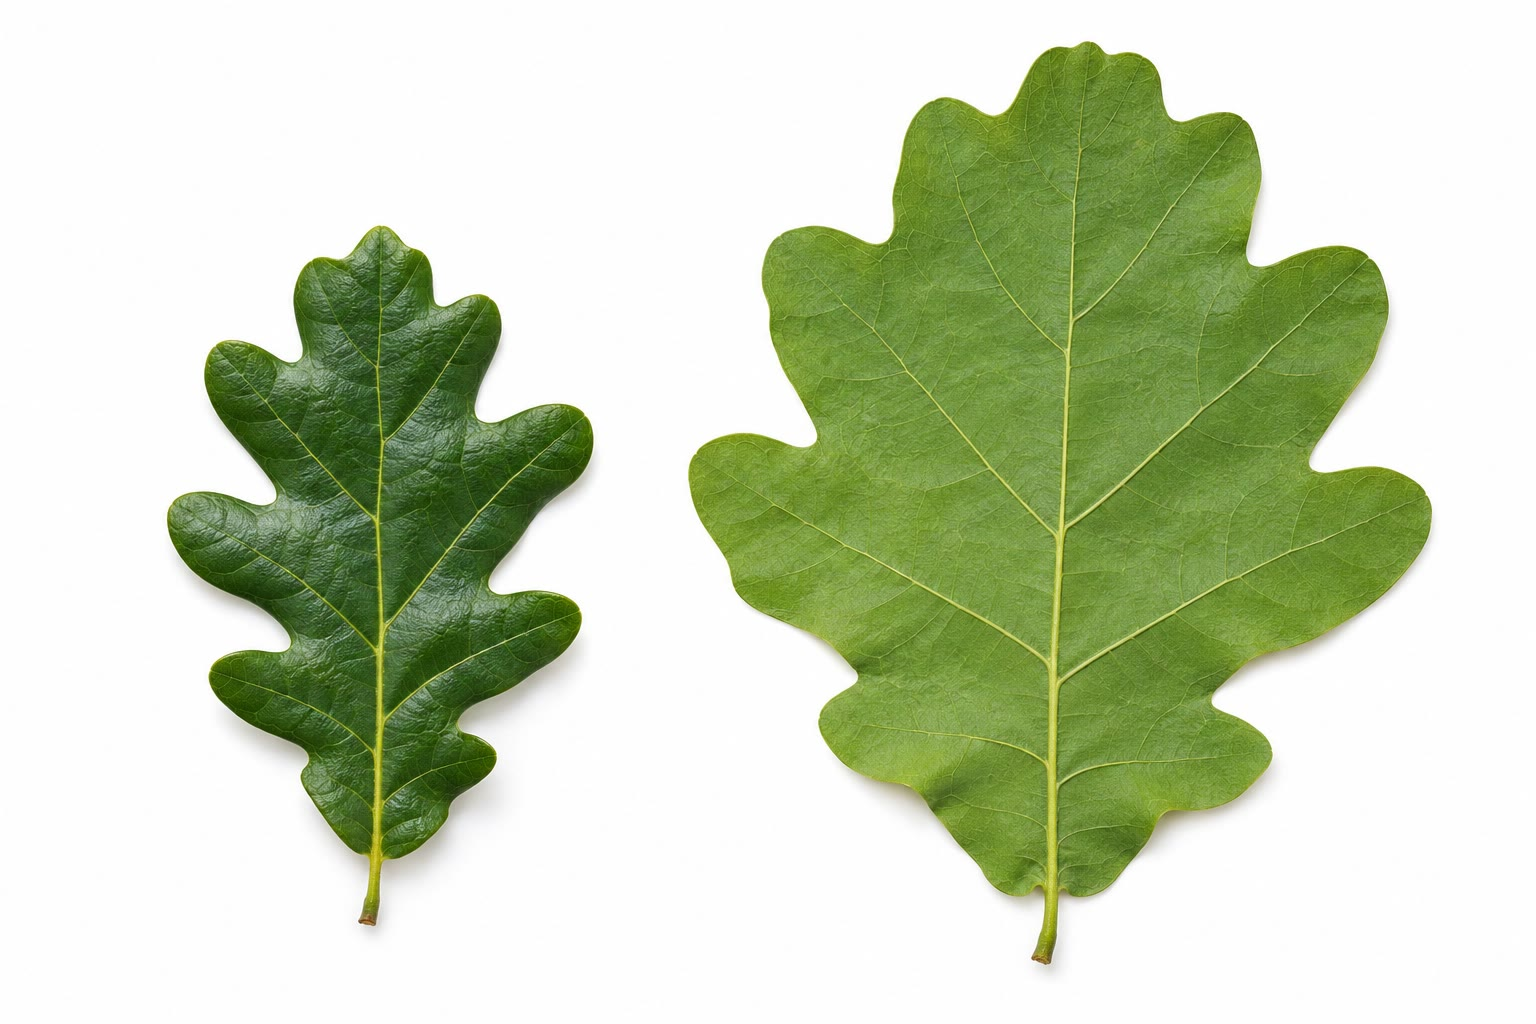
\includegraphics[width=0.55\linewidth]{images/book4/ai/b4-15-sun-shade-leaves.jpg}

{\small 同一棵橡树的\omterm{prop:b2:plant-plasticity:sunshade}{阳生叶}与\omterm{prop:b2:plant-plasticity:sunshade}{阴生叶}：\omterm{def:b2:meiosis-heredity:vocabulary}{基因型}相同，光照不同，
叶片也不同。}
\end{omfigure}

\section{读取光照}

\begin{theorem}[光敏色素作为光质计]\label{thm:b2:plant-plasticity:phytochrome}
\index{光敏色素}\index{红光与远红光之比}\index{避荫综合征}
\omterm{prop:b2:plant-flowering:photoperiod}{光敏色素}有两种形式：$P_r$ 吸收红光
（\qty{660}{nm}）并转化为 $P_{fr}$，而 $P_{fr}$
吸收远红光（\qty{730}{nm}）并转化回原来的形式——
起作用的是 $P_{fr}$。在持续光照下，两种转化达到
一种\emph{光平衡态}，其位置仅取决于
光中\omterm{thm:b2:plant-plasticity:phytochrome}{红光与远红光之比}：
\[
\varphi = \frac{P_{fr}}{P_{r} + P_{fr}} = \frac{R}{R + a\,FR},
\]
其中 $R$ 与 $FR$ 分别为两个波段的光子通量密度，
$a$ 为色素的常数（$a \approx 0.77$）。
阳光中 $R{:}FR \approx 1.15$，故 $\varphi \approx 0.6$；经叶片过滤的光，
叶片吸收红光而透过远红光，其 $R{:}FR
\approx 0.2$，故 $\varphi \approx 0.2$。低 $\varphi$ 告诉植物，
它在被遮阴之前已处于其他植株之下或之旁——
来自邻株的远红光会在朝向邻株的一侧被感知到——
于是植物作出\emph{\omterm{thm:b2:plant-plasticity:phytochrome}{避荫综合征}}的反应：
茎伸长加快，叶柄加长，叶片上举，
分枝减少，开花提前。
郁闭林冠下的幼苗，其伸长速率可增加一倍。
\end{theorem}
\begin{proof}
设 $k_1 R$ 为 $P_r \to P_{fr}$ 的速率常数（与红光通量成
正比），$k_2\,FR$ 为 $P_{fr} \to P_r$ 的速率常数。平衡时
$k_1 R\,P_r = k_2\,FR\,P_{fr}$，故 $P_{fr}/P_r = k_1 R/
(k_2 FR)$，且 $\varphi = P_{fr}/(P_r + P_{fr}) = R/(R + a\,FR)$，
其中 $a = k_2/k_1$。（两种形式在两个波段均有一定吸收，这已由
常数 $a$ 包含，结果的形式不变。）取
$a = 0.77$：$1.15/(1.15 + 0.77) = 0.60$；$0.2/(0.2 + 0.77) = 0.21$。
\end{proof}

\begin{omfigure}
\begin{tikzpicture}
\begin{axis}[
  width=0.7\linewidth, height=5.2cm,
  axis x line=bottom, axis y line=left,
  xmin=0, xmax=1.4, ymin=0, ymax=0.8,
  xlabel={光的红光与远红光之比}, ylabel={$\varphi = P_{fr}/P_{\text{总}}$},
  xlabel style={font=\small, at={(axis description cs:0.5,-0.13)}, anchor=north},
  ylabel style={font=\small},
  tick label style={font=\small}, xtick={0,0.2,0.6,1.15}, ytick={0,0.2,0.4,0.6},
  clip=false,
]
\addplot[very thick, omDef, domain=0:1.4, samples=60] {x/(x+0.77)};
\draw[dashed, gray] (axis cs:1.15,0) -- (axis cs:1.15,0.6) -- (axis cs:0,0.6); \node[font=\scriptsize, anchor=south west] at (axis cs:1.15,0.6) {开阔阳光};
\draw[dashed, gray] (axis cs:0.2,0) -- (axis cs:0.2,0.21) -- (axis cs:0,0.21); \node[font=\scriptsize, anchor=west] at (axis cs:0.25,0.15) {郁闭林冠下};
\end{axis}
\end{tikzpicture}

{\small \omterm{prop:b2:plant-flowering:photoperiod}{光敏色素}光平衡随\omterm{thm:b2:plant-plasticity:phytochrome}{红光与远红光之比}的变化。
阳光使大部分色素处于活性形式；
经叶片过滤的光则使色素大多处于非活性形式，植物借此
将此差异解读为周围有邻居。}
\end{omfigure}

\begin{proposition}[向光性]\label{prop:b2:plant-plasticity:phototropism}
\index{向光性}\index{向性}\index{乔洛德尼–温特假说}
\emph{\omterm{prop:b2:plant-plasticity:phototropism}{向性}}是一种由定向刺激引起的生长运动。
在\emph{\omterm{prop:b2:plant-plasticity:phototropism}{向光性}}中，茎向蓝光弯曲：
光在茎尖被一种蓝光受体
（向光素）感受，从茎尖向下运输的\omterm{prop:b2:plant-meristems:apical}{生长素}被重新分配
至背光一侧——其载体蛋白移至侧膜——
背光一侧因获得更多\omterm{prop:b2:plant-meristems:apical}{生长素}，
比向光一侧伸长更快，于是茎向光弯曲。
这种弯曲是差异生长，而非肌肉运动：它只发生在\omterm{prop:b2:plant-meristems:ram}{伸长区}，
历时一两小时，且不可逆。
根中同样过量的\omterm{prop:b2:plant-meristems:apical}{生长素}\emph{抑制}伸长，
因此根背光弯曲。
\end{proposition}
\begin{proof}[证据]
达尔文（1880）用禾本科植物胚芽鞘证明，尖端感受光，
其下方区域发生弯曲：
用不透光的帽子罩住尖端，弯曲即消失；
罩住基部的套管则无影响，透明帽则不影响弯曲。
博伊森-詹森（1913）切去尖端，在其间插入一块明胶：弯曲依然发生，
故信号是一种可扩散的物质；在背光一侧插入云母片可阻断弯曲，
插在向光一侧则无此作用，说明该物质是沿背光一侧向下运输的。
温特（1928）从切下的尖端收集琼脂中的物质，
将一块偏离中心的琼脂块放在黑暗中去顶的胚芽鞘上，
胚芽鞘便向远离琼脂块的方向弯曲，弯曲角度与物质量成正比；
又从单侧光照射的尖端两半分别收集琼脂，
发现背光一侧约含三分之二的\omterm{prop:b2:plant-meristems:apical}{生长素}，
向光一侧约含三分之一（布里格斯，1957，改用更好的方法）。
生长激素的横向再分配
即为\omterm{prop:b2:plant-plasticity:phototropism}{乔洛德尼–温特假说}，
该假说至今仍成立。
\end{proof}

\begin{omfigure}
\begin{tikzpicture}[every node/.style={font=\scriptsize}, >=stealth]
  \foreach \x/\lab/\cap/\bend in {0/{完整：\\弯曲}/0/1, 2.6/{遮住尖端：\\不弯曲}/1/0, 5.2/{遮住基部：\\弯曲}/2/1, 7.8/{切去尖端：\\不弯曲}/3/0, 10.4/{尖端置于明胶上：\\弯曲}/4/1} {
    \begin{scope}[xshift=\x cm]
      \fill[omExo!30] (-0.7,0) rectangle (0.7,0.2);
      \ifnum\bend=1
        \draw[very thick, omExo!70!black] (0,0.2) -- (0,1.6) .. controls (0,2.3) and (0.5,2.6) .. (0.9,2.8);
      \else
        \draw[very thick, omExo!70!black] (0,0.2) -- (0,3.0);
      \fi
      \ifnum\cap=1 \fill[black] (-0.2,2.7) rectangle (0.2,3.1); \fi
      \ifnum\cap=2 \fill[black] (-0.2,0.2) rectangle (0.2,1.5); \fi
      \ifnum\cap=3 \draw[thick] (-0.3,2.6) -- (0.3,2.6); \fi
      \ifnum\cap=4 \fill[omDef!35] (-0.2,2.55) rectangle (0.2,2.75); \draw[very thick, omExo!70!black] (0.55,2.75) -- (0.9,3.1); \fi
      \node[below, align=center] at (0,-0.15) {\lab};
    \end{scope}
  }
  \node[anchor=east, align=right, omProp!80!black] at (-1.0,2.2) {光来自 \\右侧 $\to$};
\end{tikzpicture}

{\small 胚芽鞘实验。达尔文：尖端感受光，
其下方区域弯曲；罩住尖端则弯曲停止，
遮住基部则无影响。博伊森-詹森：信号穿过
一块明胶——说明它是一种物质。}
\end{omfigure}

\begin{omfigure}
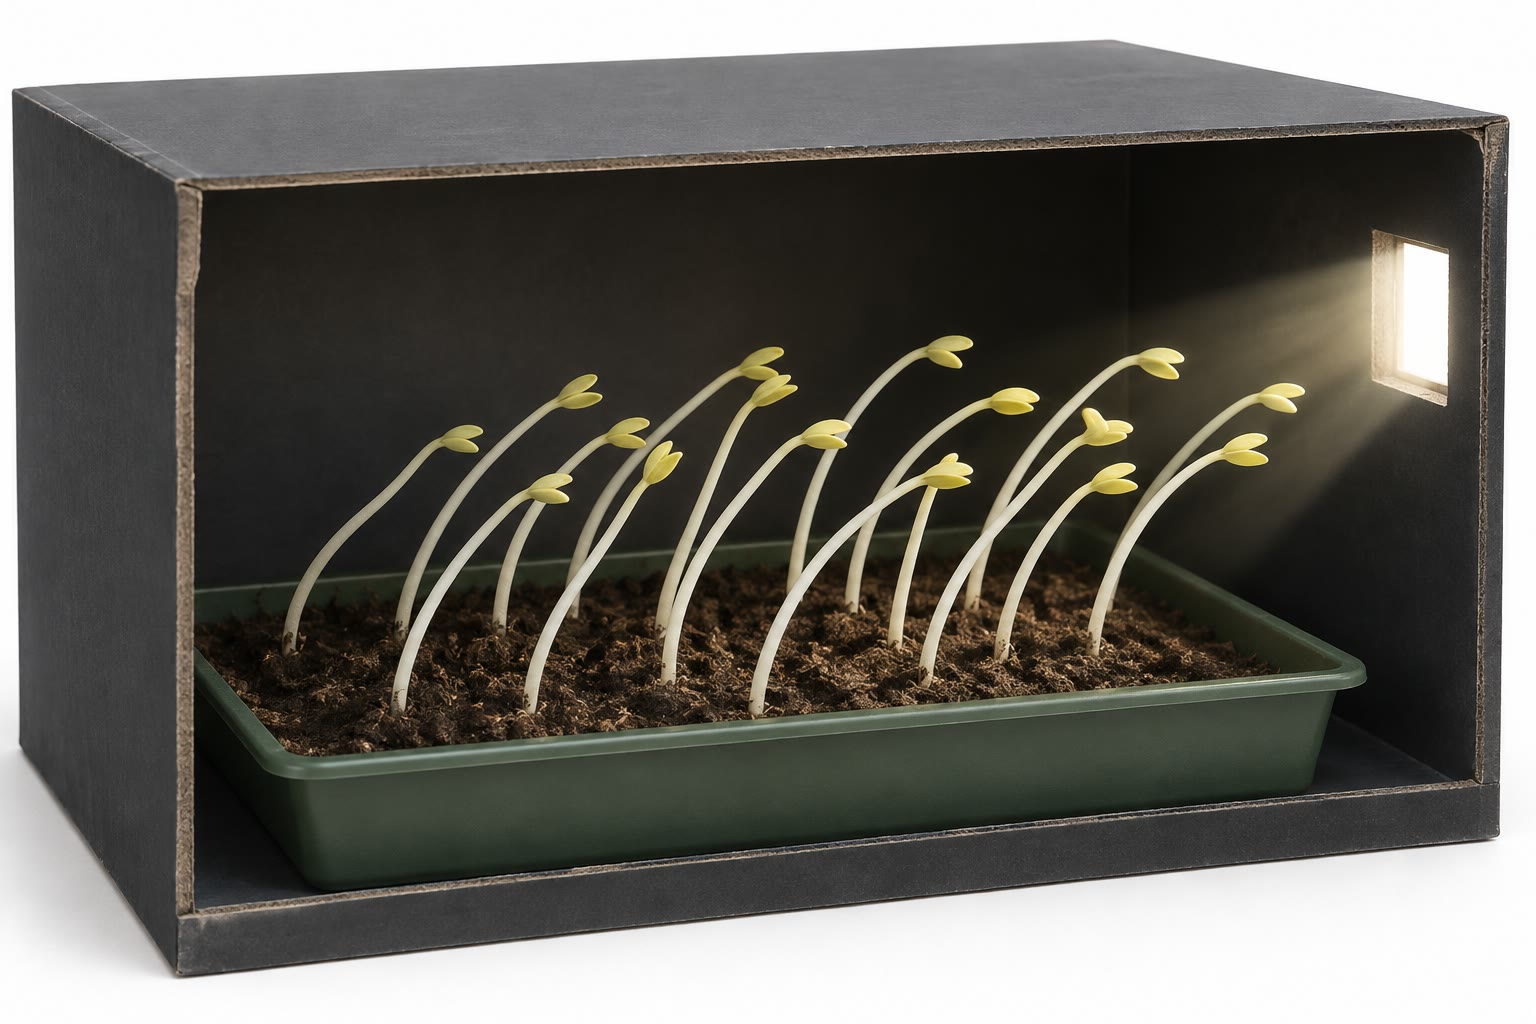
\includegraphics[width=0.55\linewidth]{images/book4/ai/b4-15-phototropism.jpg}

{\small 置于仅有一扇窗的箱中的幼苗：全部向光弯曲，
原因是背光一侧生长更快。}
\end{omfigure}

\begin{theorem}[茎的弯曲程度]\label{thm:b2:plant-plasticity:bend}
若直径为 $d$ 的茎，其背光一侧伸长的相对量为 $\varepsilon_s$，
向光一侧为 $\varepsilon_l$，在长度为 $L$ 的生长区内，
则该生长区弯曲的角度为
\[
\theta = \frac{L\,(\varepsilon_s - \varepsilon_l)}{d}
\]
（以弧度计）。某胚芽鞘以每小时 \qty{5}{\%} 的速率生长，
其生长区长 \qty{10}{mm}、直径 \qty{1}{mm}，\omterm{prop:b2:plant-meristems:apical}{生长素}按 $65 : 35$ 分配，
使两侧的生长速率分别为平均值的 $1.3$ 倍和 $0.7$ 倍，
则三小时后弯曲角度为 $\theta = 10\times(0.195 - 0.105)/1 =
0.9$ 弧度，约为 \qty{50}{\degree}。
弯曲无需新的机制：只要\cref{ch:b2:plant-meristems}中的正常生长在两侧不均等，
便已足够。
\end{theorem}
\begin{proof}
生长区的两侧成为半径分别为 $\rho + d/2$ 和
$\rho - d/2$、张角同为 $\theta$ 的圆弧，长度分别为 $L(1 +
\varepsilon_s)$ 和 $L(1 + \varepsilon_l)$；二者之差为
$\theta d$，故 $\theta = L(\varepsilon_s - \varepsilon_l)/d$。三小时内
以每小时 \qty{5}{\%} 计，平均伸长量为 $0.15$；
$1.3\times 0.15 = 0.195$，$0.7\times 0.15 = 0.105$。
\end{proof}

\begin{proposition}[向重力性]\label{prop:b2:plant-plasticity:gravitropism}
\index{向重力性}\index{平衡石}
侧放的茎与根会在
数小时内分别向上与向下弯曲。重力方向由\emph{\omterm{prop:b2:plant-plasticity:gravitropism}{平衡石}}——
即\omterm{prop:b2:plant-meristems:ram}{根冠}与茎的淀粉鞘中特化细胞内的致密淀粉粒
——会沉降到细胞下侧，
并在数秒内通过压迫膜或内质网，
改变\omterm{prop:b2:plant-meristems:apical}{生长素}载体的分布，使\omterm{prop:b2:plant-meristems:apical}{生长素}积累于
下侧。在茎中，下侧生长较快，
茎便向上弯曲；在根中，同样的\omterm{prop:b2:plant-meristems:apical}{生长素}过量抑制下侧，
上侧生长较快，根便向下弯曲。去掉
\omterm{prop:b2:plant-meristems:ram}{根冠}后，根便能向任意方向笔直生长；无淀粉的
\omterm{def:b2:genome-diversification:mutation}{突变}体感知重力的能力很差；缓慢旋转的转鼓（即随转器）上的根，
其\omterm{prop:b2:plant-plasticity:gravitropism}{平衡石}永不能沉降，
便失去方向地生长。这一反应是
对 Cholodny--Went 机制的第二种应用，只是感受器不同。
\end{proposition}

\section{水分：关闭气孔}

\begin{proposition}[气孔控制]\label{prop:b2:plant-plasticity:stomata}
\index{气孔}\index{保卫细胞}\index{脱落酸}\index{气孔导度}
叶片上的小孔，即\emph{\omterm{prop:b2:plant-plasticity:stomata}{气孔}}，各由两个
\emph{\omterm{prop:b2:plant-plasticity:stomata}{保卫细胞}}围成，其\omterm{def:b2:unicellular-diversity:prokaryote}{细胞壁}厚薄不均，因此当它们
吸收钾离子与水分而膨胀时，会向两侧弯开，使小孔张开，
失水时则关闭小孔。\omterm{prop:b2:plant-plasticity:stomata}{气孔}在
清晨，于蓝光照射且胞内 $\mathrm{CO_2}$ 浓度较低时张开，
黑暗中关闭；当\emph{\omterm{def:b2:plant-flowering:dormancy}{脱落
酸}}到达——它或来自感知土壤干旱的根，并经木质部向上运输，
或来自因失去膨压而缺水的叶片本身——以及空气十分干燥时，
\omterm{prop:b2:plant-plasticity:stomata}{气孔}都会在数分钟内关闭。\emph{\omterm{prop:b2:plant-plasticity:stomata}{气孔导度}} $g_s$
同时决定失水量 $E = g_s\,(w_i - w_a)$（即
叶内饱和水汽与空气中水汽摩尔分数之差），
以及吸入的 $\mathrm{CO_2}$ 量 $A = g_s\,(c_a -
c_i)/1.6$（其中因子 $1.6$ 为水汽与
$\mathrm{CO_2}$ 扩散系数之比）。叶片以水换碳，
通过这一个阀门，其\emph{水分利用效率}为
\[
\frac{A}{E} = \frac{c_a - c_i}{1.6\,(w_i - w_a)},
\]
每摩尔水对应的碳仅为千分之几摩尔。典型的
C$_3$ 叶片每固定一克碳需消耗 \qtyrange{400}{600}{g} 水，
C$_4$ 叶片约为其一半，CAM 植物则约为其五分之一。
\end{proposition}

\begin{omfigure}
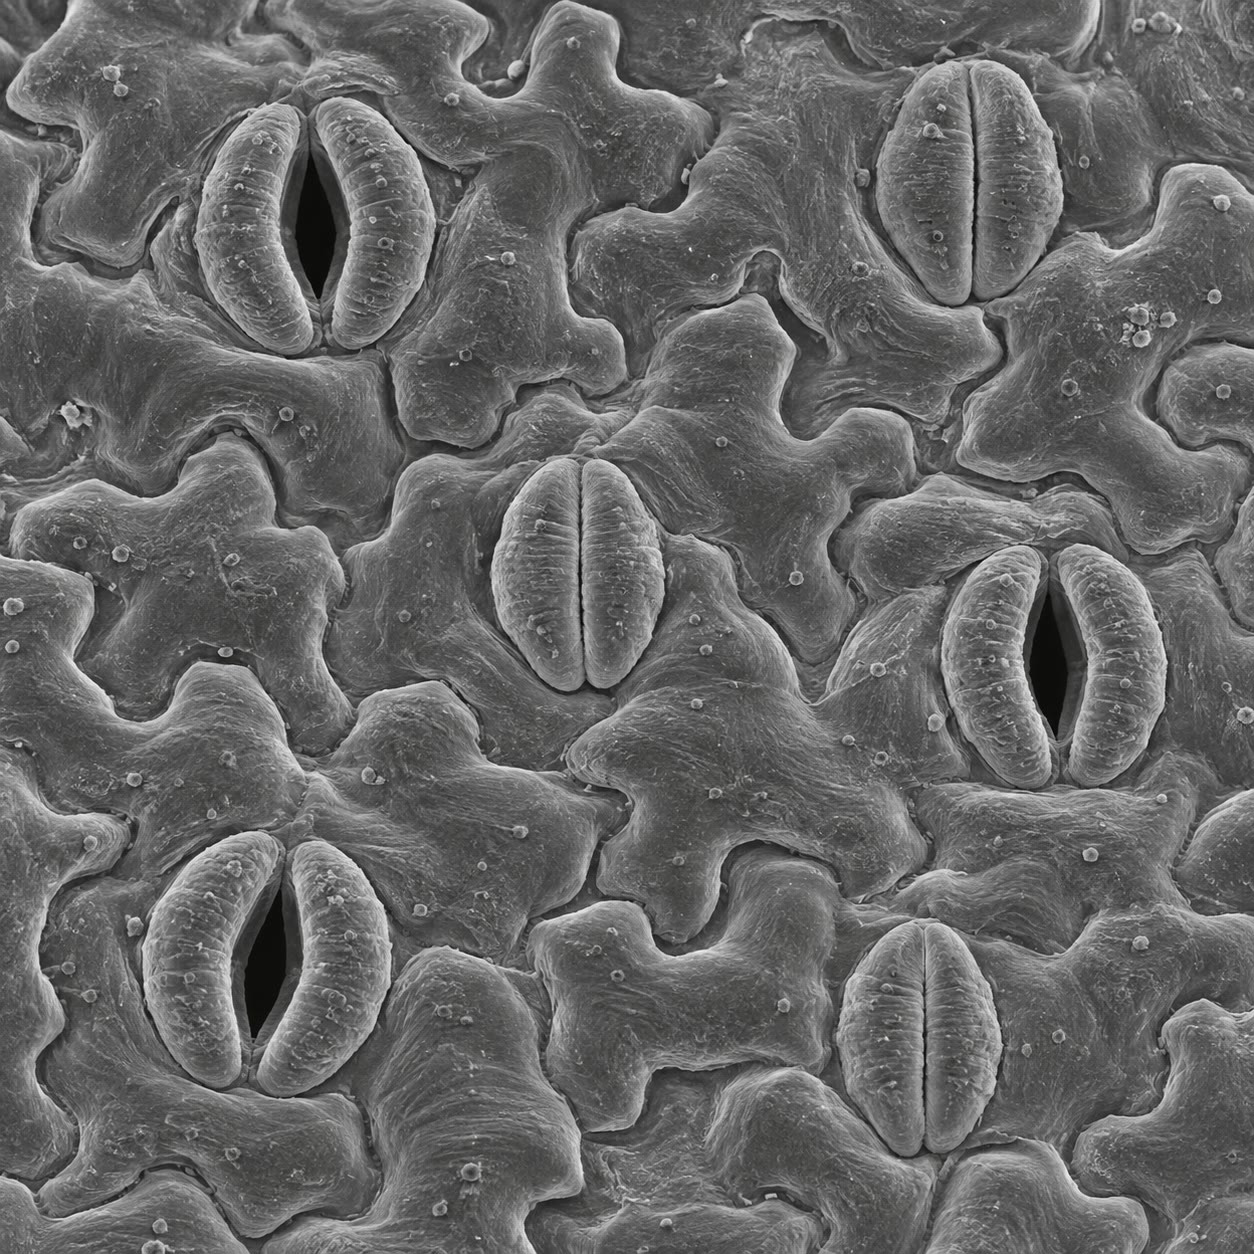
\includegraphics[width=0.42\linewidth]{images/book4/ai/b4-15-stomata-sem.jpg}

{\small 叶片背面的\omterm{prop:b2:plant-plasticity:stomata}{气孔}，有的张开、有的关闭：
每个小孔周围有两个\omterm{prop:b2:plant-plasticity:stomata}{保卫细胞}，它是叶片借以
用水换取二氧化碳的阀门。}
\end{omfigure}

\begin{example}[一天的碳成本]\label{ex:b2:plant-plasticity:wue}
正午时，一片向日葵叶，其 $g_s = \qty{0.3}{mol.m^{-2}.s^{-1}}$，
$w_i - w_a = 0.02$ 且 $c_a - c_i = \qty{120}{\micro mol/mol}$，
蒸腾量为 $E = \qty{6}{mmol.m^{-2}.s^{-1}}$，固定量为 $A =
0.3\times 120/1.6 = \qty{22}{\micro mol.m^{-2}.s^{-1}}$：$A/E =
\qty{3.7e-3}{}$，即每个碳原子对应 270 个水分子，
每克碳对应 \qty{400}{g} 水。一公顷这样的叶片
夏日一天内失水 \qty{40}{t}，以固定 \qty{100}{kg}
碳。土壤变干时，\omterm{def:b2:plant-flowering:dormancy}{脱落酸}使\omterm{prop:b2:plant-plasticity:stomata}{气孔导度}降至
此值的十分之一：$E$ 降至原来的十分之一，$A$ 的降幅
小于此（因为 $c_i$ 也随之下降），植物便以饥饿式的饮食维持生存，
而不致渴死。
\end{example}

\begin{proposition}[干旱适应]\label{prop:b2:plant-plasticity:xerophytes}
\index{旱生植物}\index{CAM 植物}\index{肉质植物}
生长于干旱环境的植物（\emph{\omterm{prop:b2:plant-plasticity:xerophytes}{旱生植物}}）综合运用可遗传的
结构与策略。减少失水：角质层加厚；\omterm{prop:b2:plant-plasticity:stomata}{气孔}
凹陷于小窝中或隐于毛下（毛可使静止空气层增厚）；
叶退化为刺（仙人掌）或在旱季脱落，小而厚的
叶片卷曲。储水：肉质茎与叶，内含保水的
黏液。扩展根系：根深达 \qty{50}{m}（牧豆树），或
在地表下横向伸展，以便吸收一场阵雨的水分。改变代谢途径：\omterm{prop:b2:plant-plasticity:xerophytes}{CAM
植物}夜间张开\omterm{prop:b2:plant-plasticity:stomata}{气孔}，此时 $w_i - w_a$ 较小，将
$\mathrm{CO_2}$ 固定为苹果酸，白天在\omterm{prop:b2:plant-plasticity:stomata}{气孔}关闭时
再将其释放并重新固定——同样的碳，只需五分之一的水。逃避：沙漠
一年生植物以\omterm{def:b2:angiosperm-reproduction:seed}{种子}形式存活数年，并在
雨后数周内完成生命周期。耐受：复苏植物失去 \qty{95}{\%} 的
水分后仍能复活。每种策略都有其代价——CAM 生长缓慢，
肉质化使植株沉重，刺则无法进行光合作用——
而付出这些代价的植物，在水分充足之处必被超越。
\end{proposition}

\begin{omfigure}
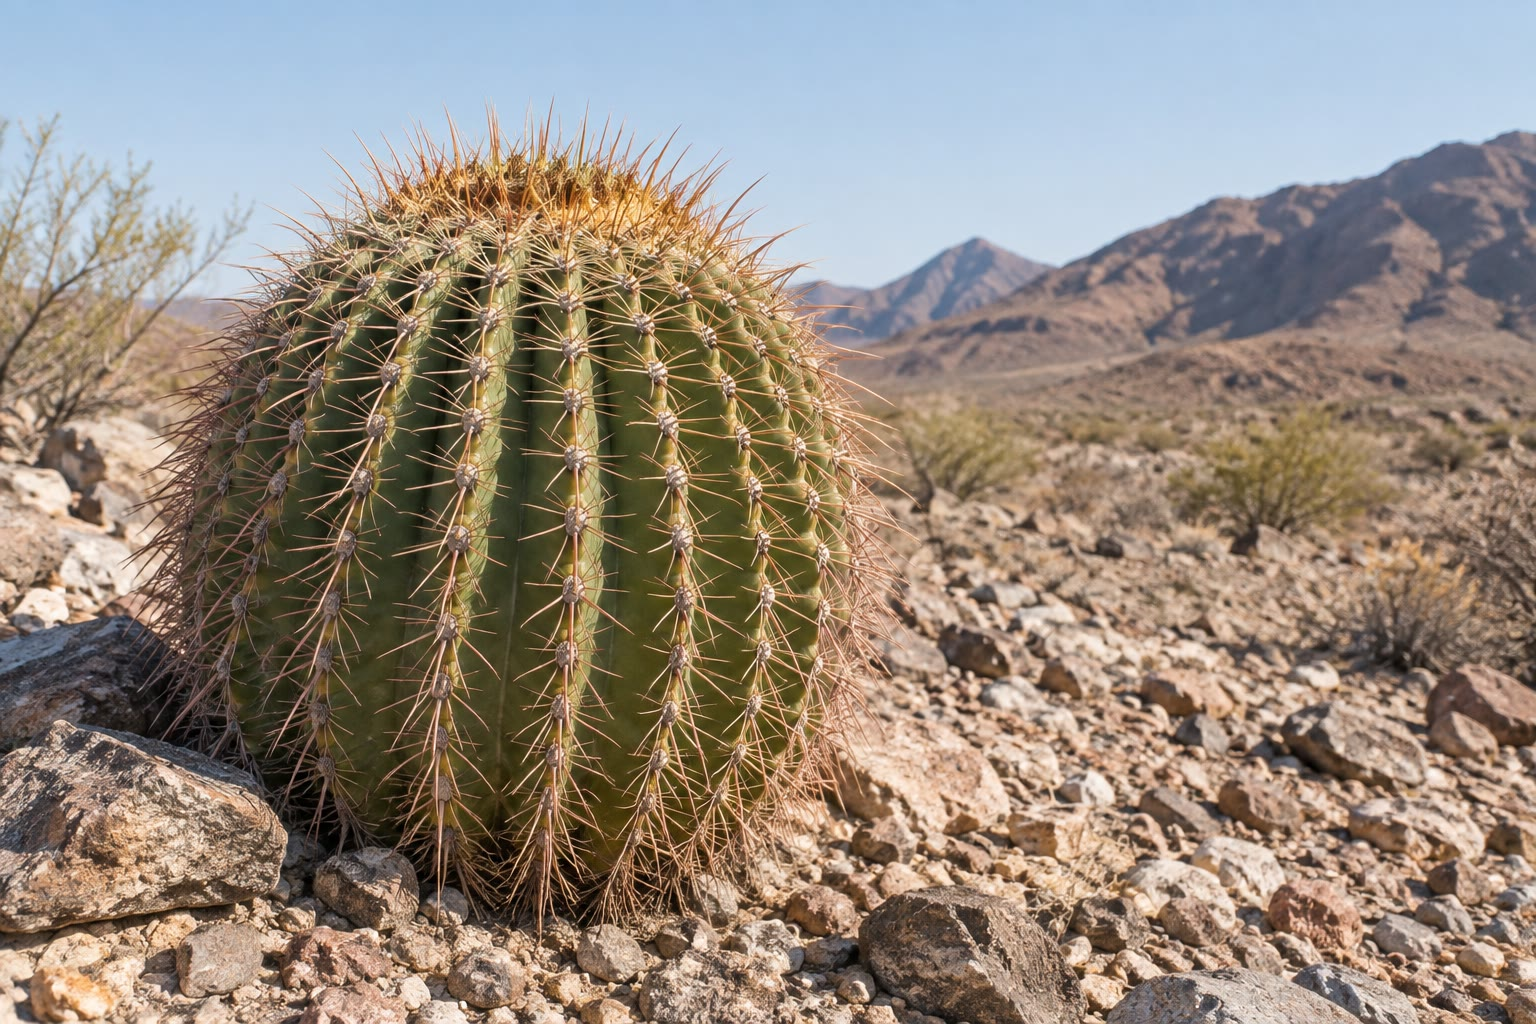
\includegraphics[width=0.55\linewidth]{images/book4/ai/b4-15-cactus.jpg}

{\small 一株桶状仙人掌：肉质茎具有厚角质层，
有利于雨后膨胀的棱，叶退化为刺，并具
仅在夜间张开的\omterm{prop:b2:plant-plasticity:stomata}{气孔}。}
\end{omfigure}

\section{低温、盐分与胁迫反应}

\begin{proposition}[胁迫驯化]\label{prop:b2:plant-plasticity:stress}
\index{低温驯化}\index{盐生植物}\index{热激蛋白}
在 \qty{4}{\celsius} 下处理一周，可使冬季黑麦的致死温度
由 \qty{-5}{\celsius} 降至 \qty{-25}{\celsius}：细胞积累了
能降低冰点并保护膜结构的糖类与蛋白质，
改变了脂质组成以保持膜的流动性，并产生
抑制冰晶生长的抗冻蛋白。导致死亡的并非
冰本身，冰在细胞间无害地形成，而是
细胞失水，水分离开细胞去结冰。在
\qty{40}{\celsius} 下数小时，即可诱导\emph{\omterm{prop:b2:plant-plasticity:stress}{热激蛋白}}，它们
使变性蛋白重新折叠，并在
\qty{45}{\celsius} 下保护细胞。盐分的应对方式有：根部排斥，
将盐分区隔于液泡中（以相容性溶质在
细胞溶胶中加以平衡），以及在真正的\emph{\omterm{prop:b2:plant-plasticity:stress}{盐生植物}}中，
经盐腺将盐分排出。上述大多数反应都经过同一
信号通路：感受器、胞质钙离子浓度升高、\omterm{def:b2:plant-flowering:dormancy}{脱落酸}，
以及一组\omterm{prop:b2:cell-differentiation:transcriptional}{转录因子}，它们开启数百个
保护基因——一种与动物免疫反应同样普遍的胁迫程序，
并且和免疫反应一样代价高昂：驯化后的植物
生长缓慢；在无需驯化时仍驯化的植物，会输给
不这样做的植物。
\end{proposition}
\begin{proof}[证据]
\omterm{prop:b2:plant-plasticity:stress}{低温驯化}实验测定叶片中半数细胞死亡的
温度（LT$_{50}$），分别在低温处理前后测定；
这一变化在一周内可达十至二十度，
并可由一周的温暖逆转。无法开启低温程序的\omterm{def:b2:genome-diversification:mutation}{突变}体
（CBF \omterm{prop:b2:cell-differentiation:transcriptional}{转录因子}）驯化能力很差，而组成型表达这些因子的植物
无需驯化即可抵御霜冻，
——但生长为侏儒。
\end{proof}

\begin{omfigure}
\begin{tikzpicture}[every node/.style={font=\scriptsize}, >=stealth]
  \node[draw, rounded corners, fill=omExo!25, align=center] (s) at (0,0) {胁迫 \\干旱、低温、\\盐、高温};
  \node[draw, rounded corners, fill=omDef!15, align=center] (sen) at (3.2,0) {感受器 \\（膜、膨压、\\未折叠蛋白）};
  \node[draw, rounded corners, fill=omDef!15, align=center] (ca) at (6.4,0) {第二信使 \\Ca$^{2+}$、ABA};
  \node[draw, rounded corners, fill=omProp!20, align=center] (tf) at (9.6,0) {转录 \\因子};
  \node[draw, rounded corners, fill=omThm!15, align=center] (out) at (12.8,0.9) {保护性基因：\\溶质、抗冻蛋白、\\分子伴侣、转运蛋白};
  \node[draw, rounded corners, fill=omThm!15, align=center] (out2) at (12.8,-0.9) {生长减缓：\\代价};
  \draw[->, thick] (s) -- (sen); \draw[->, thick] (sen) -- (ca); \draw[->, thick] (ca) -- (tf);
  \draw[->, thick] (tf) -- (out); \draw[->, thick] (tf) -- (out2);
\end{tikzpicture}

{\small 植物胁迫响应的共同模式：一个感受器、一个
钙与\omterm{def:b2:plant-flowering:dormancy}{脱落酸}信号、\omterm{prop:b2:cell-differentiation:transcriptional}{转录因子}，以及一套
保护基因程序——以生长为代价。}
\end{omfigure}

\begin{example}[误导的线索]\label{ex:b2:plant-plasticity:lie}
可塑性的好坏完全取决于线索。处于邻居远红光遮阴下的幼苗
会伸长——若邻居是幼苗，这样做是对的，
它能超过邻居；若邻居是树，则是致命的，因为用于茎的储备
被根和叶夺走。密植作物彼此遮阴、
伸长并倒伏；育种者已选出小麦与水稻，
它们对远红光信号不作反应。二月的温暖一周使叶片展开，
三月的霜冻将其冻死；存活下来的植株是
那些同时也会计入低温的植株（见\cref{ch:b2:plant-flowering}）。
每种可塑性反应都是对线索诚实性的一次押注，而
\omterm{def:b2:plant-plasticity:plasticity}{反应规范}的形状，取决于该谱系过去
线索说真话的频率。
\end{example}

\section{练习}

\begin{exercise}[$\star$]\label{exo:b2:plant-plasticity:1}
定义\omterm{def:b2:plant-plasticity:plasticity}{表型可塑性}、\omterm{def:b2:plant-plasticity:plasticity}{反应规范}、\omterm{def:b2:plant-plasticity:plasticity}{驯化适应}与
适应，并各举一个植物实例。
\end{exercise}

\begin{exercise}[$\star$]\label{exo:b2:plant-plasticity:2}
描述达尔文的四种胚芽鞘处理及各自的结果。
\end{exercise}

\begin{exercise}[$\star$]\label{exo:b2:plant-plasticity:3}
列出\omterm{prop:b2:plant-plasticity:sunshade}{阳生叶}与\omterm{prop:b2:plant-plasticity:sunshade}{阴生叶}之间的五项差异，并说明
这一选择在叶片生命周期的哪个阶段做出。
\end{exercise}

\begin{exercise}[$\star$]\label{exo:b2:plant-plasticity:4}
\omterm{prop:b2:plant-plasticity:stomata}{气孔}如何张开？早晨是什么使其张开，
干旱时又是什么使其关闭？
\end{exercise}

\begin{exercise}[$\star\star$]\label{exo:b2:plant-plasticity:5}
计算 $\varphi$，取 $R{:}FR = 1.15$（全光照）、$0.7$（林隙）、$0.2$
（冠层下）及 $0.05$（深阴）的值，并取 $a = 0.77$。在
这四种条件中，哪两者之间植物会开启避荫反应，若阈值为
$\varphi = 0.4$？
\end{exercise}

\begin{exercise}[$\star\star$]\label{exo:b2:plant-plasticity:6}
某叶片的 $g_s = \qty{0.25}{mol.m^{-2}.s^{-1}}$，$w_i - w_a = 0.025$，
$c_a - c_i = \qty{100}{\micro mol/mol}$。计算 $E$、$A$、
水分利用效率（分别以摩尔和每克碳所对应的水克数表示），
以及 12 小时白天内每平方米的失水量。
\end{exercise}

\begin{exercise}[$\star\star$]\label{exo:b2:plant-plasticity:7}
对一株 CAM 植物重算上一题，其\omterm{prop:b2:plant-plasticity:stomata}{气孔}在夜间开放，
取 $w_i - w_a = 0.005$，导度不变。碳的水分代价
降低了多少倍？
\end{exercise}

\begin{exercise}[$\star\star$]\label{exo:b2:plant-plasticity:8}
\omterm{prop:b2:plant-plasticity:gravitropism}{平衡石}是半径为 \qty{2}{\micro m} 的淀粉粒，
密度为 \qty{1500}{kg/m^3}，位于密度为 \qty{1100}{kg/m^3}
、动力黏度为 \qty{0.01}{Pa.s} 的细胞质中。计算其沉降速度（斯托克斯）和
穿过一个 \qty{10}{\micro m} 细胞所需的时间。为何回转仪
每分钟转动一次，就能消除向重性？
\end{exercise}

\begin{exercise}[$\star\star$]\label{exo:b2:plant-plasticity:9}
一根直径为 \qty{2}{mm} 的茎，每小时生长 \qty{2}{\%}，
作用于 \qty{20}{mm} 长的区段。单侧光使\omterm{prop:b2:plant-meristems:apical}{生长素}以 $60 : 40$ 分配。
两小时后它弯曲了多大角度？经过多长时间，它
才与原来的方向成 \qty{90}{\degree}？
\end{exercise}

\begin{exercise}[$\star\star\star$]\label{exo:b2:plant-plasticity:10}
储备物质为 \qty{50}{mg} 的幼苗，开阔处每天伸长 \qty{2}{cm}，
冠层下每天伸长 \qty{4}{cm}，茎伸长超出叶片供应的部分，
每厘米耗费 \qty{1}{mg} 的储备物质。
在荨麻丛中，冠层高出它 \qty{30}{cm}，
在林中则为 \qty{10}{m}。在哪种情形下避荫反应
能够成功，另一种情形下会怎样？
\end{exercise}

\begin{exercise}[$\star\star\star$]\label{exo:b2:plant-plasticity:11}
解释为何凝固通过脱水而非冰晶杀死细胞，
一周的低温如何防止这种情况，以及为何
全年都表达低温程序的植株会成为侏儒。
\end{exercise}

\begin{exercise}[$\star\star\star$]\label{exo:b2:plant-plasticity:12}
“可塑性是对线索可靠性的一次押注。”请结合远红光信号、
二月的温暖一周，以及培育出的
不理会邻居的作物，加以讨论。
\end{exercise}

\section{问题：冠层下的幼苗}

\begin{problem}[{周末问题——幼苗的光照环境，
伸长、水分收支与向性，依据其感受器的物理过程计算，
最终求其光敏色素状态及两周后的株高，
以及每日耗水量}]
\label{pb:b2:plant-plasticity:1}
一株桦树幼苗在冠层下萌发，该冠层透过
\qty{3}{\%} 的阳光，并将 $R{:}FR$ 由 $1.15$ 降至 $0.2$
（$a = 0.77$）。全日照下，它每天伸长 \qty{1.5}{cm}；
在冠层下，其伸长速率乘以 $1 +
2(0.6 - \varphi)$。茎直径为 \qty{2}{mm}，生长区长
\qty{15}{mm}。叶面积共 \qty{20}{cm^2}；$g_s =
\qty{0.2}{mol.m^{-2}.s^{-1}}$；阴影中 $w_i - w_a = 0.015$，
林隙中为 $0.03$；$c_a - c_i = \qty{80}{\micro mol/mol}$；白天
长 \qty{14}{h}。\omterm{prop:b2:plant-plasticity:gravitropism}{平衡石}：半径 \qty{2.5}{\micro m}，密度
\qty{1500}{kg/m^3}，置于密度为 \qty{1100}{kg/m^3} 的细胞质中，
黏度为 \qty{0.01}{Pa.s}。

\medskip
\noindent\textbf{第一部分——光照。}
\begin{enumerate}
  \item 计算开阔处与冠层下的 $\varphi$。
  \item 幼苗由 $\varphi$ 得出什么结论，
        若冠层透光 \qty{3}{\%} 而不改变光色，
        （即遮阳网），幼苗又会作何结论？
  \item 计算冠层下的伸长速率。
  \item 在该处生长 14 天后，此幼苗与
        开阔处的同胞苗相比有多高？
  \item 一侧出现林隙，使该侧的 $R{:}FR$ 升至
        $0.8$。会引起哪两种反应？分别由哪两种
        光感受器介导？
  \item 冠层下发育的叶片为何更大、更薄，
        若冠层被砍伐，它们会怎样？
\end{enumerate}

\medskip
\noindent\textbf{第二部分——向林隙弯曲。}
\begin{enumerate}[resume]
  \item 林隙处的光使\omterm{prop:b2:plant-meristems:apical}{生长素}在茎的两侧按 $65 : 35$ 分配，
        取第 3 题中冠层下的伸长速率，
        计算一小时内生长区两侧各自的
        相对伸长量。
  \item 计算一小时后的弯曲角度。
  \item 经过多长时间茎会直指林隙，
        若林隙与竖直方向成 \qty{60}{\degree}？
  \item 茎现已倾斜。计算一个\omterm{prop:b2:plant-plasticity:gravitropism}{平衡石}的沉降速度，
        以及穿过一个 \qty{12}{\micro m} 细胞所需的时间。
  \item 茎的重力\omterm{prop:b2:plant-plasticity:phototropism}{向性}与\omterm{prop:b2:plant-plasticity:phototropism}{向光性}现已相互矛盾。
        在避阴植物中何者占优，这样做为何
        具有适应意义？
  \item 同一幼苗的一条根在石块作用下
        倾斜了 \qty{45}{\degree}。预测其反应，并说明
        它为何与茎的反应方向相反，尽管二者机制相同。
\end{enumerate}

\medskip
\noindent\textbf{第三部分——水分。}
\begin{enumerate}[resume]
  \item 计算阴影中每平方米的蒸腾速率，
        以及幼苗叶片一天失去的水量。
  \item 计算每平方米每秒及每天固定的碳量，
        以及以每克碳所耗水的克数表示的
        水分利用效率。
  \item 幼苗在阴影中一天的全部碳获得量为多少，
        以毫克计？
  \item 重新计算林隙中失去的水量与效率。
  \item 土壤变干，\omterm{def:b2:plant-flowering:dormancy}{脱落酸}使 $g_s$ 降至
        \qty{0.02}{mol.m^{-2}.s^{-1}}。重新计算 $E$ 与 $A$
        （假设 $c_a - c_i$ 升至 \qty{200}{\micro mol/mol}）。
        哪一个下降得更多？为什么？
  \item 幼苗有 \qty{5}{g} 叶片组织，含水量为 \qty{85}{\%}，
        在萎蔫前可失去其中的五分之一。
        若根不供给任何水分，\omterm{prop:b2:plant-plasticity:stomata}{气孔}保持开放，
        它在林隙中能维持多久？
  \item 解释为何 CAM 策略不适合桦树幼苗
        在冠层下生长。
\end{enumerate}

\medskip
\noindent\textbf{第四部分——赌注。}
\begin{enumerate}[resume]
  \item 幼苗储有 \qty{100}{mg} 储备物质。在阴影中，每厘米茎
        超出其叶片供给部分的每厘米茎耗费 \qty{2}{mg}，
        若只靠储备物质，它能建成
        多长的茎？
  \item 冠层是上方 \qty{40}{cm} 处的荨麻丛；另一种情形是
        上方 \qty{8}{m} 处的林木。在每种情形下，判断伸长
        能否在储备耗尽前达到光照，并说明
        在林木中更好的反应应为何。
  \item 桦树是开阔地的先锋植物；山毛榉幼苗则
        可在深阴中等待数十年。比较二者
        关于 $\varphi$ 的预期\omterm{def:b2:plant-plasticity:plasticity}{反应规范}。
  \item 一位植物育种者希望培育一种密植作物，
        使其不发生伸长。你会使哪一种感受器或反应失效，
        又必须检查哪一种副作用？
  \item 用两句话解释：为何一株无法感知邻近植物的植物，
        与一株总是相信邻近植物的植物，
        都不如一株有时感知、有时不感知的植物。
  \item 给出结论：阳光下与阴影中的 $\varphi$，幼苗
        14 天后的株高，以及阴影中的每日耗水量，
        与林隙中的每日耗水量。
\end{enumerate}
\end{problem}
